\chapter{Realizzazione interfaccia grafica}
Una volta generati i modelli predittivi per effettuare nuove analisi, ho pensato che creare questo modello senza poi poterne usufruire come un applicativo vero e proprio sarebbe risultato fine a sé stesso.

Ho quindi scelto di creare una semplice interfaccia grafica attraverso la quale poter effettuare delle predizioni sullo stato d’animo della persona ripresa da una webcam.

Una volta avviato il programma per l’interfaccia grafica, si presenta una schermata che dà la possibilità di scegliere fra i modelli predittivi creati \ref{fig:image16}

\begin{figure}
    \begin{center}    
        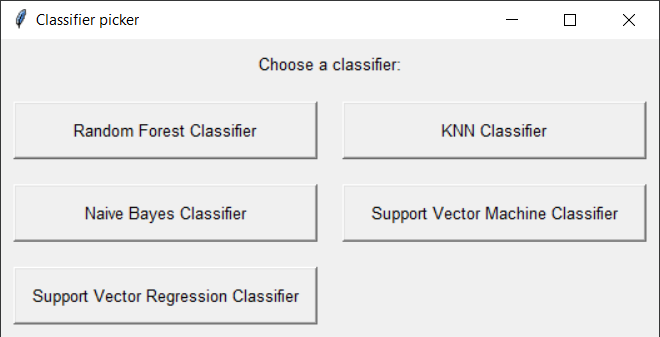
\includegraphics[width=0.9\linewidth]{images/image51.png}
        \caption{Prima schermata interfaccia}
        \label{fig:image16}
    \end{center}
\end{figure}

Una volta scelto l’algoritmo da utilizzare, questo viene, se precedentemente utilizzato, prelevato dalla memoria, altrimenti viene generato al momento e poi salvato su file binario attraverso i metodi disponibili nella libreria pickle (utilizzata sia per la scrittura che per la lettura di questi file contenti i modelli).
\begin{minted}[bgcolor=bg]{python}
def getRandomForestClassifier():
    filePathRandomForestClassifier = join(
        dirname(abspath(__file__)), 
        "randomForestClassifier.pickle"
    )

    if isfile(filePathRandomForestClassifier):
        with open(filePathRandomForestClassifier, "rb") as f:
            randomForestClassifier = pickle.load(f)
    else:
        print("Creazione random forest classifier")
        randomForestClassifier = RandomForestClassifier(
            n_estimators=100, 
            verbose=True, 
            random_state=42
        )
        Xtrain, yTrain, Xtest, yTest = getXtrainYTrainXtestYTest()
        randomForestClassifier.fit(Xtrain, yTrain)

        with open(filePathRandomForestClassifier, "wb") as f:
            pickle.dump(randomForestClassifier, f)
        
        relativeTestResult = randomForestClassifier.score(Xtest, yTest)
        print("Relative test result:", relativeTestResult)

    return randomForestClassifier
\end{minted}
La schermata che si presenta successivamente è riportata a \ref{fig:image17}.
\begin{figure}
    \begin{center}    
        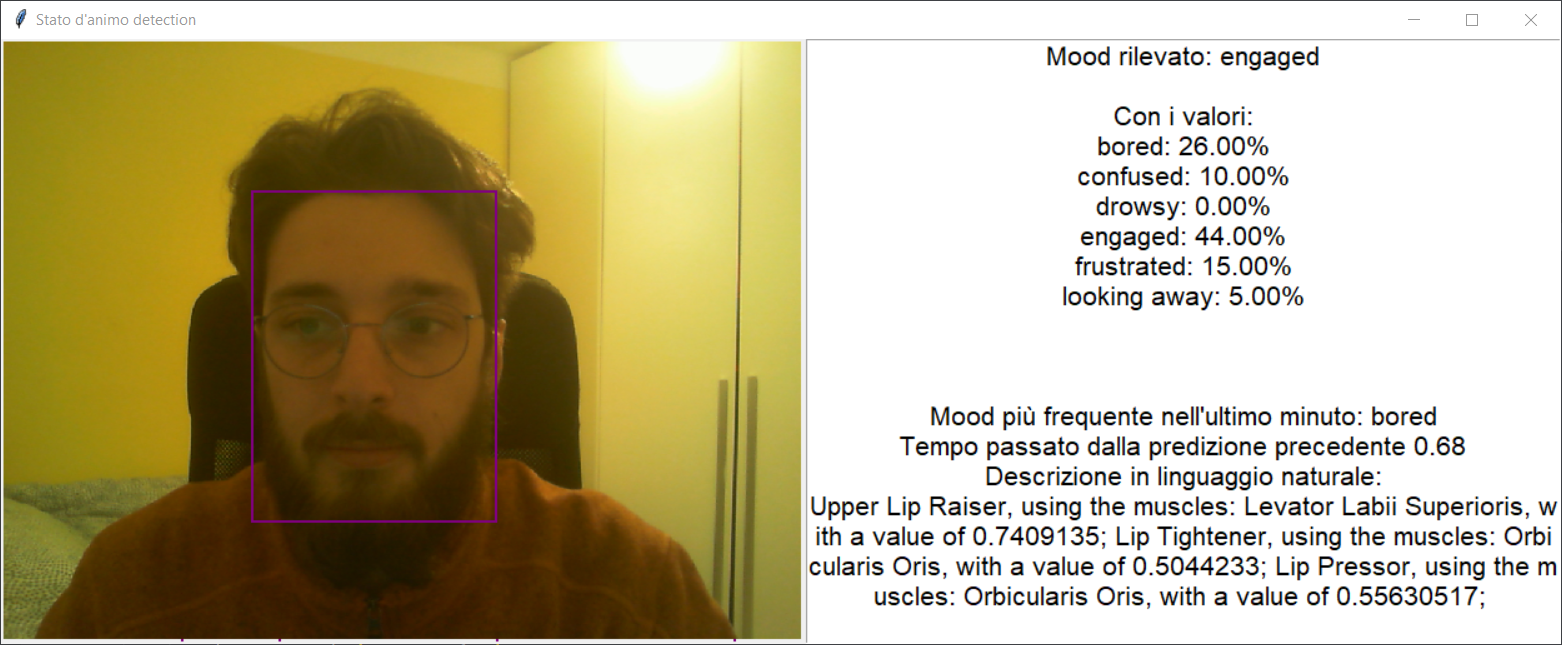
\includegraphics[width=0.9\linewidth]{images/image52.png}
        \caption{Schermata rilevazione mood}
        \label{fig:image17}
    \end{center}
\end{figure}

Sulla sinistra è possibile notare la webcam dalla quale vengono estratti i frame per effettuare le analisi e che riprende, ovviamente, il soggetto di fronte alla fotocamera.

Sulla destra è invece possibile osservare il testo, suddiviso in:

La prima riga, dove è presente il mood rilevato, ossia la label con la percentuale di predizione più alta, secondo il modello predittivo precedentemente scelto, sull’immagine che è stata catturata in quel momento.

Subito sotto sono presenti tutte le label e le relative percentuali di predizione calcolate.

È poi riportato il mood più frequente nell’ultimo minuto; per decidere quale label fra quelle estratte vada riportata qui ho immagazzinato in una struttura dati dizionario (dict di python) ognuna delle label, con la relativa percentuale di predizione più alta, raccolte nell’ultimo minuto, e le ho utilizzate come chiave; come valori ho invece immagazzinato il timestamp nel quale è stata effettuata la predizione.

Ogni minuto questo dizionario viene aggiornato rimuovendo le coppie chiave valore prelevate più di un minuto prima. 
\begin{minted}[bgcolor=bg]{python}
def addToBestClassesLastMinute (bestClass):
    bestClassesLastMinute[time.time()] = bestClass

def removeOldKeys(bestClassesLastMinute):
    currentTime = time.time()
    oneMinuteAgo = currentTime - 60
    return {
        k:v for k,v in bestClassesLastMinute.items() if k > oneMinuteAgo
    }
\end{minted}
Viene inoltre mostrato quanto tempo è passato fra una predizione e l’altra, così da fornire un’idea delle prestazioni del programma.

Infine, viene mostrata la descrizione in linguaggio naturale generata dall'immagine.

Ovviamente le prestazioni dell’interfaccia variano in base alla macchina sulla quale viene compilata:

il personal computer che ho utilizzato per eseguire il programma, dotato di queste specifiche:
\begin{itemize}
    \item Ryzen 7 5800H
    \item 16GB ram DDR4
    \item GeForce RTX 3060 6GB (mobile)
    \item SSD m.2
\end{itemize}

mi ha permesso di ottenere intorno alle 100 predizioni al minuto e, di fatti, il video mostrato nella schermata risulta andare a scatti.

È importante mettere in luce che per effettuare le predizioni l’immagine mostrata sullo schermo viene salvata sul disco, e che le prestazioni dipendono anche dal tipo di disco sul quale viene eseguita l’analisi; ho difatti riscontrato un decremento notevole delle performance nel momento in cui ho provato ad eseguire il programma su un hard disk classico rispetto ad un SSD, tipologia di disco utilizzata in entrambe le macchine sopracitate.

Un’altra differenza importante è data dal fatto che la macchina presentata è dotata di una scheda video Nvdia che può quindi sfruttare la tecnologia CUDA per effettuare l’estrazione delle Action Units dall’immagine prelevata, il che migliora esaurientemente le prestazioni.

Effettuando delle predizioni impostando il parametro del costruttore della classe Detector, offerta da py-feat, a “cpu” ho rilevato un decremento di performance, che porta il delta tempo fra una predizione e l’altra da poco meno di un secondo ($\sim$0.6/0.7s) a $\sim$1.6/1.7 secondi.
